\documentclass[12pt,oneside,a4paper,parskip]{scrbook}
\usepackage[utf8]{inputenc}
\usepackage{csquotes}
\usepackage[T1]{fontenc}
\usepackage{floatflt}
\usepackage{subfigure}
\usepackage[pdftex]{graphicx}
\usepackage[hidelinks]{hyperref}
\usepackage{color}
\usepackage{amssymb}
\usepackage{textcomp}
\usepackage{nicefrac}
\usepackage{scrhack}
\usepackage{pdfpages}
\usepackage{float}
\usepackage{pdflscape}
\usepackage{subfigure}
\usepackage{pdfpages}
\usepackage[verbose]{placeins}
\usepackage[markcase=ignoreuppercase,headsepline,plainfootsepline]{scrlayer-scrpage}
\usepackage{listings}
\usepackage{xcolor}
\usepackage{color}
\usepackage{caption}
\usepackage{subfigure}
\usepackage{epstopdf}
\usepackage{longtable}
\newlength\colw
\usepackage{booktabs}
\usepackage{nameref}

\usepackage[
  style=ext-authoryear,
  backend=biber, 
  maxbibnames=1000,
  maxcitenames=3,
  maxalphanames=2,
  introcite=plain,
  ]{biblatex}
\DeclareFieldFormat{bbx@introcite}{\mkbibbold{\mkbibbrackets{#1}}}
\renewcommand*{\introcitepunct}{\addspace}


\DefineBibliographyStrings{ngerman}{
    andothers={et\ al\adddot}
} % aus u.a. zu et al. machen

\DeclareLabelalphaTemplate{
  %\labelelement{
  %  \field[final]{shorthand}
  %  \field{label}
  %  \field[strwidth=4,strside=left,uppercase=true,noalphaothers=true]{labelname}
  %}
  %\labelelement{
  %  \field[strwidth=2,strside=right]{year}
  %}
  \labelelement{
    \field{author}
  }
  \labelelement{
    \field{ }
  }
  \labelelement{
    \field{year}
  }
}
\usepackage{setspace}
\onehalfspacing
\usepackage{seqsplit}
\usepackage{hhline}

\bibliography{bibliography}


%%%%%%%%%%%%%%%%%%%
%% definitions
%%%%%%%%%%%%%%%%%%%
\def\BaAuthor{Achim Winter}
\def\BaAuthorStudyProgram{Computer Science}
\def\BaType{Bachelor thesis}
\def\BaTitle{Operating a Smartphone as a Hardware Security Module}
\def\BaSupervisorOne{Prof.\ Dr.\ Junker-Schilling}
\def\BaSupervisorTwo{Prof.\ Dr.\ Huffstadt}
\def\BaDeadline{14.02.2020}

\ifdefined\iswithfullname
  \def\ShowBaAuthor{\BaAuthor}
\else
  \def\ShowBaAuthor{N.~N.}
\fi

\hypersetup{
pdfauthor={\ShowBaAuthor},
pdftitle={\BaTitle},
pdfsubject={Subject},
pdfkeywords={Keywords}
}

%%%%%%%%%%%%%%%%%%%
%% configs to include
%%%%%%%%%%%%%%%%%%%
\colorlet{punct}{red!60!black}
\definecolor{background}{HTML}{EEEEEE}
\definecolor{delim}{RGB}{20,105,176}
\colorlet{numb}{magenta!60!black}

\definecolor{gray}{rgb}{0.4,0.4,0.4}
\definecolor{darkblue}{rgb}{0.0,0.0,0.6}
\definecolor{cyan}{rgb}{0.0,0.6,0.6}

\definecolor{pblue}{rgb}{0.13,0.13,1}
\definecolor{pgreen}{rgb}{0,0.5,0}
\definecolor{pred}{rgb}{0.9,0,0}
\definecolor{pgrey}{rgb}{0.46,0.45,0.48}

\lstset{
  basicstyle=\ttfamily,
  columns=fullflexible,
  showstringspaces=false,
  commentstyle=\color{gray}\upshape
  linewidth=\textwidth
}

\usepackage{array}
\newcolumntype{C}[1]{>{\centering\let\newline\\\arraybackslash\hspace{0pt}}m{#1}}   % center
\newcolumntype{L}[1]{>{\raggedright\let\newline\\\arraybackslash\hspace{0pt}}m{#1}} % left
\newcolumntype{R}[1]{>{\raggedleft\let\newline\\\arraybackslash\hspace{0pt}}m{#1}}  % right
%\newcolumntype{w}[1]{>{\raggedleft\hspace{0pt}}p{#1}}

\lstset{language=Java,
  showspaces=false,
  showtabs=false,
  tabsize=1,
  breaklines=true,
  keepspaces=true,
  numbers=left,
  numberstyle=\scriptsize,
  stepnumber=1,
  numbersep=8pt,
  showstringspaces=false,
  breakatwhitespace=true,
  commentstyle=\color{pgreen},
  keywordstyle=\color{pblue},
  stringstyle=\color{pred},
  basicstyle=\ttfamily,
  backgroundcolor=\color{background},
%  moredelim=[il][\textcolor{pgrey}]{$$},
%  moredelim=[is][\textcolor{pgrey}]{\%\%}{\%\%}
}

\newcommand*{\forcetwosidetitle}[1][1]{%
 \begingroup
   \cleardoubleoddpage
   \KOMAoptions{titlepage=true}% useful e.g. for scrartcl
   \csname @twosidetrue\endcsname
   \maketitle[{#1}]
 \endgroup
}


\begin{document}


%%%%%%%%%%%%%%%%%%%
%% Titelseite
%%%%%%%%%%%%%%%%%%%


\frontmatter
\titlehead{%  {\centering Seitenkopf}
  {University of applied Sciences W\"{u}rzburg-Schweinfurt\\
   Faculty of Computer Science and Business Informatics}}
\subject{\BaType}
\title{\BaTitle\\[15mm]}
\subtitle{\normalsize{submitted to the University of Applied Sciences W\"{u}rzburg-Schweinfurt in the Faculty of \BaAuthorStudyProgram}}
\author{\ShowBaAuthor}
\date{\normalsize{Submitted on: \BaDeadline}}
\publishers{
  \normalsize{First Supervisor: \BaSupervisorOne}\\
  \normalsize{Second Supervisor: \BaSupervisorTwo}\\
}
%\lowertitleback{
% \centering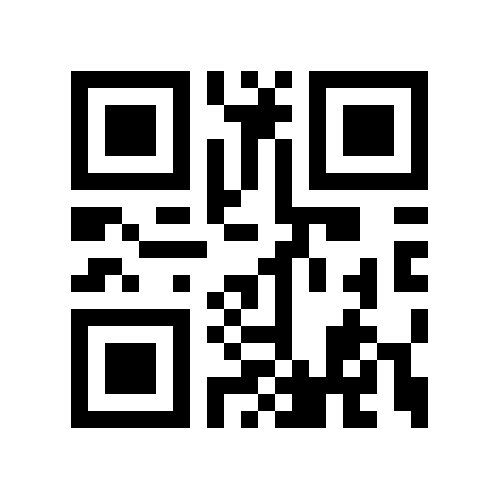
\includegraphics[width=4cm]{qrcode-thesis.png}

%}
\forcetwosidetitle


%%%%%%%%%%%%%%%%%%%
%% abstract
%%%%%%%%%%%%%%%%%%%

\section*{Abstract}
Managing private keys on different devices is currently very complicated. Especially if this is has to be done in a secure way. In addition, every device that is in possession of the private key constitutes another security risk for attacks. 

Manufacturers of mobile phones are adding more and more security features to their products. The latest standards of these security features even offer an independent Hardware Security Module, which works encapsulated from the actual device on its own chip. Therefore, it will also be investigated how secure the respective solutions are.

This will then be used to show how the smartphone can manage the secrets securely and make them available for other devices or applications.



\section*{Zusammenfassung}
Die Verwaltung von privaten Schlüsseln auf unterschiedlichen Geräten ist derzeit sehr kompliziert. Vor allem, wenn das auch noch auf eine sichere Art und Weise geschehen soll. Außerdem bildet jedes Gerät, welches im Besitz des privaten Schlüssel ist, ein weiteres Sicherheitsrisiko für Angriffe. 

Dabei fügen Hersteller von Mobilfunkgeräten immer mehr Sicherheitsmerkmale in ihre Produkte ein. Die neusten Standards dieser Sicherheitsmerkmale bieten gar ein eigenständiges Hardware Security Module, welches abgekapselt vom eigentlichen Gerät auf einem eigenen Chip arbeitet. Daher soll auch untersucht werden, wie sicher die jeweiligen Lösungen sind.

Damit soll dann gezeigt werden, wie das Smartphone die Geheimnisse sicher verwalten kann und sie für andere Geräte bzw. Anwendungen verfügbar machen kann.

\newpage
\chapter*{Acknowledgment}

I would like to thank Prof. Dr. Junker-Schilling for his helpful support. The seminars and the discussions with the other students helped me a lot to stay on schedule and make the work what it is now. My further thanks go to Prof. Dr. Huffstadt for the second supervision. 

I would also like to thank Francis Pouatcha and Steffen Blümm for their support from adorsys. The discussions always brought new ideas on how the work can be further improved. Thank you very much for that.

I would also like to thank my proofreaders and my family. Thanks to you too, the work has become what it is today.

%%%%%%%%%%%%%%%%%%%
%% Inhaltsverzeichnis
%%%%%%%%%%%%%%%%%%%
\tableofcontents



%%%%%%%%%%%%%%%%%%%
%% Main part of the thesis
%%%%%%%%%%%%%%%%%%%
\mainmatter

\chapter{Introduction}\label{ch:intro}

The two main fields of cryptography in computer systems can be divided between symmetric-key cryptography and public-key cryptography. Symmetric-key utilizes the same key for the sender and the receiver, which was the first form of encryption and also secure and easy to understand. If this is done by close relatives this may be possible, but exchanging this key to every website when browsing through the Internet is impractical. Not only because it is physically nearly impossible, but also because the amount of keys one would have to store securely would be growing by the square of number of communication partners.
To avoid this kind of key management, Whitfield Diffie and Martin Hellman published a system in 1976 known as the public-key cryptography. With this system it is possible to generate an encryption key over an insecure network such as the Internet in order to secure subsequent communication. However, the real encryption key is never transferred to the opposing communication partner. In fact the real encryption key is being calculated by using public and private keys, which have a mathematical relation to each other. Each communication partner has to create a pair of his own private and public key. While the public key can be exposed to the Internet, the private key has to remain secret. 
By using both key pairs, a common shared key can be calculated which then can be used for the encryption. This system relies on the computational complexity, such as prime factorization, which is hard to do with big numbers \parencite{luber_encryption_2017}.
%[Was ist der Diffie-Hellman-Schlüsselaustausch?] [https://en.wikipedia.org/wiki/Cryptography#Computer_era]

The usage of encryption when visiting a web page has grown from about 30\% in 2014 to about 80\% by the end of 2019

\begin{figure}[ht]
	\centering
  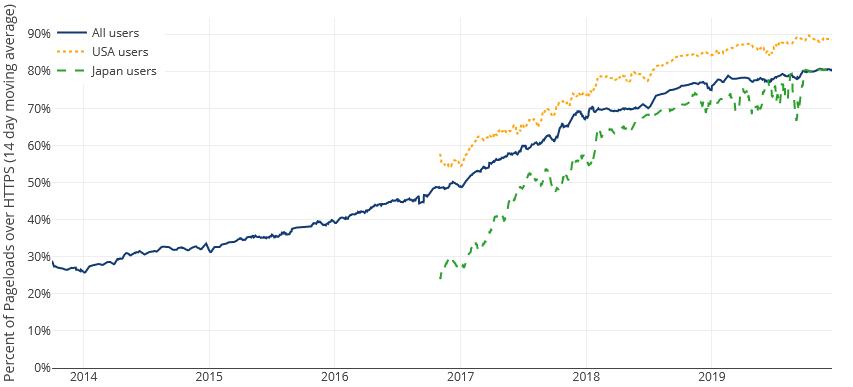
\includegraphics[width=0.8\textwidth]{ressources/https_statistics.png}
	\caption{Percentage of Web Pages Loaded by Firefox Using HTTPS \parencite{letsencrypt_lets_2019}}
\end{figure}
\newpage
There are also worldwide discussions about the development of 5G mobile technology. Huawei, the manufacturer of the required hardware, is suspected of having installed interception capabilities for the Chinese state \parencite{stokel-walker_banning_2019}. \newline
In addition, browser manufacturers like Mozilla or Google warn their users when they visit a website without HTTPS with an open red lock next to the address bar \parencite{google_milestone_2018}.

This shows that the use of encryption is becoming increasingly important, since it must always be assumed that data transmitted unencrypted over the Internet will be read by someone.

\section{Motivation}

The use of public/private keys that are not handled automatically is too troublesome for many people, even IT professionals. The manual distribution of keys between several devices becomes more difficult the more devices there are. However, using end-to-end encryption with multiple devices is only possible if they have access to the same private key. The synchronization of private keys is often done via cloud providers, although they are also often attacked. The keys would either have to be additionally encrypted, which makes handling more difficult again, or distributed in another way. On the other hand, systems such as Android or iOS offer more and more security features in their latest versions, such as the generation of random numbers in their own encapsulated processor. It is therefore worth investigating to what extent this can be used to simplify the handling of private keys.

\section{Objective}

The goal of this work is to use a smartphone as a kind of secure wallet to store private keys on it. The private keys should never leave the smartphone. However, the smartphone must make the services of the private keys available to other applications, such as an email client on a desktop computer, so that encrypted emails can be read from there.

\section{Environment}

The work was carried out in cooperation with adorsys GmbH \& Co. KG. Founded in 2006, adorsys primarily offers software services in the banking and insurance industries. Adorsys became particularly well known in the european banking scene through the open source implementation of the PSD2 payment directive, which came into force in 2019. The largest customers include Teambank AG, Datev eG, Bankverlag and ERGO Direkt. Adorsys has thus built up expertise in the financial sector, where security plays a major role. 

%\section{Structural Overview}

\chapter{Approach}

\section{Analysis of the current situation}

First, it is necessary to examine how keys are currently handled and their most common uses, where the end user needs to be able to access the keys. Use cases like Diffie-Hellman are not considered, because the normal user has no interaction with them.

\section{Requirements for Key-Distribution Systems}

After the frequent use cases have been identified, an analysis can be made of the requirements they place on key management. 

\section{Concept}

From the results of the requirements, a concept can be worked out how different systems can work together to best meet the requirements and provide the user with the best possible user experience. 

\section{Implementation}

With the help of the concept, a prototype can then be developed in the Implementation chapter, which fulfills the main functions of the concept exemplary. The findings that become visible during the development of the prototype can then be used to further improve the result of the work.

% Wahrscheinlich sollte man noch GRPC erklären
\chapter{Fundamentals}

\section{Quick-Response Codes}

Quick Response Codes (QR-Codes) are a kind of further development of barcodes, as they can be found on many products. Compared to barcodes, QR codes offer two dimensions instead of just one, which enables readers to read the codes faster and more robustly from different perspectives, but also contain more data. When a QR-Code reader starts to analyze the code, it first calculates the ratio between the dark and light areas and then eliminates any possible distortion. Then the modules can be viewed, holding data ready to be used again \parencite{Sangeeta_qr_2016}.

\section{Certificate Authority}
\label{sec:CA}

A Certificate Authority (CA) is an organization that creates digital certificates. The CA establishes a connection between a person or an organization and a public key. To create this connection, the CA must be able to check and confirm the identity of the person/organization. The public key is then signed, which allows other entities that trust the CA to be sure that it is the specified person/organization \parencite{luber_ca_2018}.

%\section{Phishing}

\section{S/MIME}
Secure/Multipurpose Internet Mail Extensions (S/MIME) is one of the two main ways, how mail encryption can be accomplished. It is based on public-key cryptography. S/MIME can also be used to sign mails in order to clearly identify the sender of the message and also ensures, that the message has not been manipulated. 
Otherwise this is easily possible and has already led to great damage through scamming in the past. However, if the mail is only signed instead of encrypted, it can still be read by anyone who receives the data \parencite{villadiego_dangers_2017}.

S/MIME can also be classified into four different classes. The higher the class, the more certain the recipient can be that the sender it is really the person in question.
\begin{itemize}
    \item Class 1: The CA only assures the authenticity of the mail address
    \item Class 2: In addition to Class 1, the name of the person and, if applicable, the company
    \item Class 3: Data provided from Class 2 is confirmed by official documents
    \item Class 4: Applicants must be physically present when the application is submitted
\end{itemize}

SMIME certificates can be signed by multiple CA's. There are two possibilities for signing the keys. The first is that a CA gets the order to generate a new key pair, then sign it, hand it over to the customer and delete the keys (especially the private key) after completion. However, the customer cannot verify that the private key has been deleted or has not been copied before, so he cannot be sure that only he is in possession of the private key. The other possibility is to generate the keys locally and create a Certificate Signing Request as explained in section \ref{sec:CSR} \parencite{luber_smime_2018}.

According to the principle of public-key cryptography, the private key of a user is used for signing and decrypting and the public key for encrypting and verifying a message.

\section{Certificate Signing Request}
\label{sec:CSR}

To have a certificate signed where a key pair already exists, a Certificate Signing Request (CSR) can be created. The advantage is that the private key does not have to be transferred to a CA but can remain secret. To do this, the customer must create a CSR to which information such as the common name (CN) is added. The CSR can then be signed using the customer's private key and sent to a CA to be signed. The CA then creates a digital certificate that the customer can distribute to communication partners \parencite{publico_ssl-grundlagen_2017}.

\section{Elliptic Curve Cryptography}

Elliptic curve cryptography (ECC) is also based on the system of public-key cryptography. In comparison to other public-key cryptography systems such as RSA, algorithms that work with elliptic curves require a smaller key length, which requires less computing power, but provides the same level of security, because the mathematical problem is harder to solve. It can be used for creating and verifying signatures, but not for encryption. However, it can be combined with a Diffie-Hellman Key Exchange. In this way, encryption can also be implemented \parencite{sullivan_relatively_2013}.

\subsection{DH-Key Exchange using ECC}
To perform a key exchange, both parties must commit themselves to a predetermined elliptic curve and select a common random point on the curve. From this point, a tangent can then be constructed that intersects the curve at a new point. This point is then mirrored over the X axis and selected as the new starting point. Both partners then each take a different random number and repeat this process as often as the random number indicates. The random number can then be used as a private key and remains secret. The resulting point (with its x and y values) is the public key that can be transmitted to the communication partner. As an attacker, it would now be difficult to guess how often a new point was constructed. Afterwards both parties repeat the calculation of the tangents and the corresponding points with the number of passes of their private key. Finally, both should come to the same end point, which is then the shared secret and can be used as a key for a symmetric encryption or as a input for a Key Derivation Function (KDF). However, this is only a very simplified representation. In reality there are some other things to consider, for example that the curve is not complete, but is also broken down to predetermined points with a kind of modulo operation, as in RSA \parencite{sullivan_relatively_2013}.
\begin{figure}[ht]
 \centering
 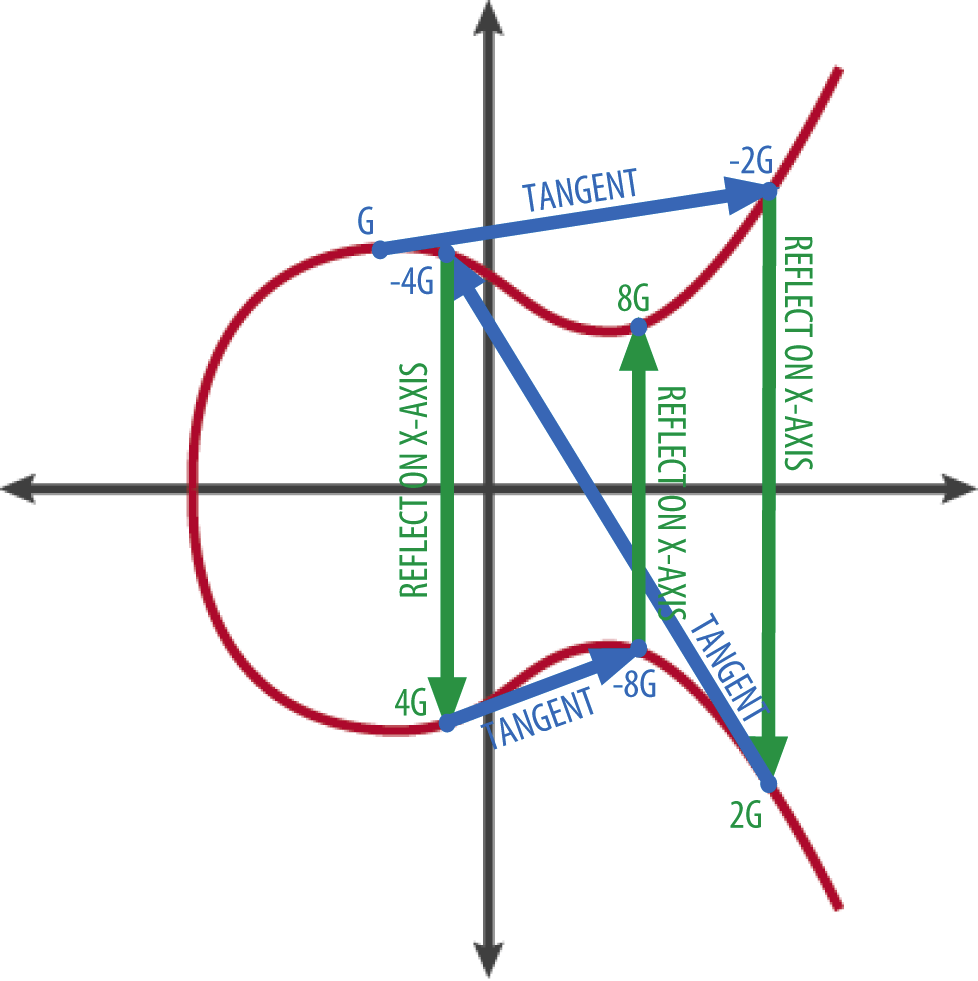
\includegraphics[width=0.8\textwidth]{ressources/ecc.png}
 \caption{Elliptic Curve Key Generation \parencite{uszak_elliptic_2017}}
 \label{fig:ecc}
\end{figure}

There are concerns that a back door has been built into one of the random number generators on a curve which was created by the NSA (NIST-P256). Other curves like X25519 or X448 that are not based on this  random number generator are considered secure \parencite{schneier_essays_2007}.

\section{ARM TrustZone}
\label{arm:TrustZone}

The ARM-TrustZone is an implementation for a Trusted Execution Environment (TEE) for ARM-Cortex based processors, which is the standard for mobile phones. It is a technology which creates two environments, a trusted and a non-trusted, simultaneously on a single cpu-core. In each of the environments, an own operating system is running. Software can run either in the trusted environment or the non-trusted. However, both environments can work together. For example an application running in the non-trusted environment can use a library which is running in the trusted environment. So, the TrustZone allows the secure storage of sensitive information like biometric information or Digital Rights Management material, even if applications in the non-trusted environment are compromised \parencite{fowler_trustzone_2017}.

\section{Hardware Security Module}
\label{sec:HSM}

A Hardware Security Module (HSM) is a peripheral device which, depending on the model, performs various cryptographic functions for another computer system. This may include: securely generating or managing cryptographic keys, protecting signatures and identities or establishing secure communication channels. It is important to note that the system using the functions of the module has no influence on the module, but can only call the functions. Such modules range from small USB tokens, such as the Ledger Nano S for crypto currency storage, to stand-alone servers that perform these cryptographic functions for a complete data center and are in addition certified for e.g. GDPR or HIPAA. As the name suggests, an HSM has separate hardware, as opposed to a Trusted Execution Environment as implemented by the ARM TrustZone. This usually consists of a CPU, a separated secure storage and a generator for random numbers \parencite{sustek_hardware_2011}.
% \parencite{ibm_hardware_2020} \parencite{gemalto_safenet_2020} 
% \section{Secure Element}

\section{Android Keystore System}
The Android Keystore is a secure environment that is used to generate and encrypt keys and prevent their extraction as much as possible. To prevent extraction, the Android Keystore follows several paths. 
In the default case, the keys are created with the help of the TrustZone and thus hardware backed. Which has some advantages as mentioned later. If this is not possible, a software fallback is used. However, both variants have very different characteristics. In general it is possible to create keys via the keystore, which can then be used directly or can be used to encrypt other things like tokens.
The Keystore can also be used to specify exactly which applications should have access to the Keystore \parencite{google_android_2020}.

\subsection{Hardware Backed Keystore}
\label{android:HWB}

With the different generations of Android versions, the Keystore System also has evolved. While smartphones certified for Android versions prior to 'Marshmallow' (Android Version 6.0) only supported the creation of signatures, verification and generating/importing of asymmetric keys, newer versions (> Android 6.0) also support the usage of symmetric keys. In addition, the keys can be generated with hardware support, if the device has an implementation of the \nameref{arm:TrustZone}. This is usually the case, if the device contains a fingerprint scanner or has access to DRM material. The device can then perform cryptographic operations with the help of the hardware backed keys. \parencite{google_hardware-backed_2020}.


\subsection{Strongbox Keystore}
\label{subsec:strongbox}
% Die Secure CPU muss zwingend eine seperate hardware CPU sein
% Theoretisch kann der Hardwarehersteller oder OEM dann auch scheiße bauen, aber die Strongbox bleibt sicher
As an extension to the \nameref{android:HWB}, Google introduced a new security feature in Android Pie (Android Version 9.0), the StrongBox Keystore. The addition is, that the kind of Keystore implementation is specified by Google. With the \nameref{android:HWB}, every mobile phone manufacturer can choose their own implementation. Also, the StrongBox must operate on separated hardware to fulfill the specifications of a \nameref{sec:HSM} and to increase the security level by using dedicated hardware.

%% HW-Backed = various implementations like TrustZone
%% StrongBox = separated hardware

\section{iOS}

\subsection{iOS Secure Enclave}
\label{subsec:sec_enclave}

Like the \nameref{subsec:strongbox}, the Secure Enclave is a coprocessor, which runs cryptographic operations.It is also in the possession of an own random-number generator, memory, operating-system and an encrypted storage. Thus, it can securely store keys, even if the kernel of the smartphone has been compromised. Also, cryptographic keys are never exposed to applications or the operating system of the main processor. Apple has this chip or a successor model of it in all smartphones and tablets since the iPhone 5S, iPad Air and iPad mini 2 \parencite{apple_storing_2020}.

\subsection{Keychain}
The iOS Keychain helps developers and users to store passwords or other sensible information. But also keys, or things like certificates. There is also a built-in password manager that is designed for the user. The way it works is that a secret which has to be stored gets packaged in a Keychain item. Additionally, there should be packaged public attributes like a name or an identifier to make the item searchable. 

\begin{figure}[ht]
  \centering
  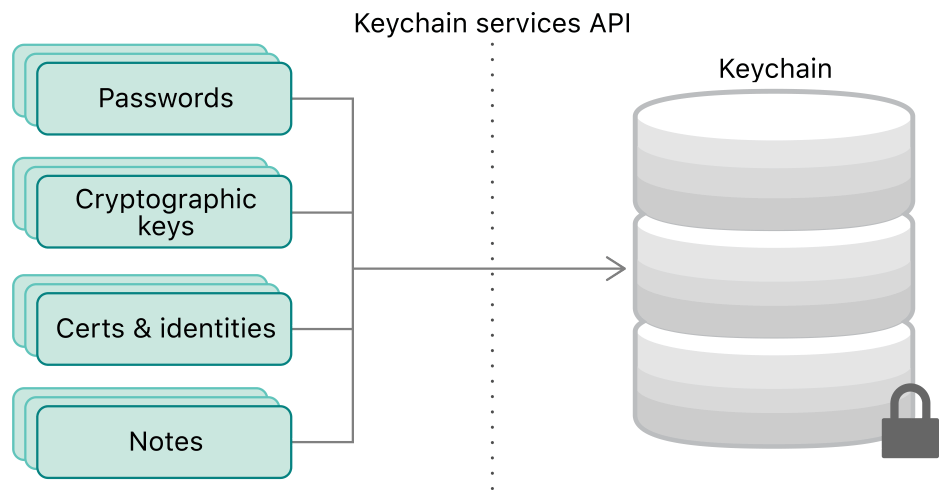
\includegraphics[width=0.8\textwidth]{ressources/apple_keychain.png}
  \caption{Apple Keychain \parencite{apple_keychain_2020}}
  \label{apple:keychain}
\end{figure}

It is an encrypted file in which all information that is particularly worth protecting is stored. In addition, this file can be synchronized via iCloud, Apple's cloud service, to make it available on all Apple devices of a user. Particularly for the iPhone, every App can create its own Keychain. Access to the Keychain can be additionally secured by authentication methods like FaceId or TouchId.

However, this means that the key was handled to some point in plaintext in the phone's memory, which could lead to a compromised key, if the app or the access to the encryption key is compromised. To mitigate this problem, Apple created the \nameref{subsec:sec_enclave} \parencite{apple_keychain_2020}.

%\subsection{Apple CryptoKit}

%Since Version 13.0, Apple introduced a new cryptographic API for developers, the CryptoKit. The intention behind this is to simplify the use of cryptographic functions for developers. The most important functions are the generation and comparison of secure digests, public-key cryptography for digital signatures, as well as the execution of DH key exchange and the generation and use of symmetric keys. Also, it is possible to use private keys which are managed and generated by the Secure Enclave.

\section{Signal-Protocol}

The signal protocol was developed by the Open Whisper Systems Foundation for their own messenger service Signal. It is an open standard end-to-end encryption protocol. The major benefit compared to other end-to-end encryption protocols is that messages can be sent encrypted even if the recipient is not online. This was also the reason for other messenger services such as WhatsApp, Skype or Facebook Messenger to implement a customized version of this encryption. Compared to other protocols, it limits the damage very well if one of the participants is compromised, since very short-lived keys are used. As explained in \nameref{subsec:double_ratchet}. The authenticity of the participants is guaranteed by the \nameref{subsec:x3dh} protocol \parencite{protocol_introducing_2018}.
% Deniability



%\parencite{cohn-gordon_formal_2017}
% Quelle dafür das andere das auch eingebaut haben.

\subsection*{Key Distribution Center}
\label{subsec:KDC}

The Key Distribution Center exists to allow users to upload multiple Key Bundles so that they can be used by other users and in addition, messages that cannot be delivered at this point, because e.g. the receiver mobile phone is switched off, are stored there temporarily until they can be sent.

\subsection{Extended Triple Diffie-Hellman --- X3DH}
\label{subsec:x3dh}

The Key Agreement Protocol knows three parties. Alice, who would like to talk to Bob, Bob who wants other parties like Alice to allow communicating with him and a server, which acts as the \nameref{subsec:KDC}.
If the private key is not explicitly mentioned, the public key is meant. The keys needed for this key exchange are as follows:
\begin{itemize}
  \item Alice's identity key $   (IK_{A})  $
  \item Alice's ephemeral key $   ({EK_{A}})  $
  \item Bob's identity key $   ({IK_{B}})  $ 
  \item Bob's signed prekey $   ({SPK_{B}})  $ 
  \item Bob's one-time prekey $   ({OPK_{B}})  $
\end{itemize}

Each of these keys is a key pair generated using elliptic curves (X25519 or X448). However, each of Bob's one-time prekeys can only be used once and Alice's ephemeral key is generated anew in each key exchange run.
The Key Agreement Protocol is built upon the Diffie-Hellman (DH) Key Exchange Protocol. The Extended Triple Diffie-Hellman (X3DH) is using three phases of the key agreement:
\begin{itemize}
  \item Bob uploads his identity key and several prekey bundles to a server.
  \item Alice requests one prekey bundle of Bob from the server.
  \item Bob receives a message from Alice and processes it.
\end{itemize}

After Alice receives the prekey bundle from the server, she checks the signature of the prekey. In the case that the signatures do not match, the protocol is aborted.
Otherwise, the three Diffie-Hellman rounds are performed, which give the protocol its name. The first round calculates a shared secret from the identity key of Alice and the signed prekey of Bob. For the second DH round, Alice must generate another ephemeral key pair using her $ {EK_{A}} $. Afterwards, the second round can be completed using Bob's identity key. This allowed both partners to verify the authenticity of each other. To provide Forward Secrecy in the protocol, the last Diffie Hellman round is then calculated using the ephemeral key of Alice and the signed prekey of Bob. 
For the option that Alice has received a one-time prekey from the server, an additional fourth round is calculated. This includes again the Ephemeral Key of Alice and the One-Time Prekey of Bob.
Finally, the results of the respective rounds can be put into a KDF, which forms the shared secret. Then Alice deletes the results of the respective rounds and her private ephemeral key. This ensures both authenticity and forward secrecy. Subsequently, she calculates an associated data byte sequence which contains the identity keys of herself and Bob.
Finally, she can generate a message containing the following keys:
\begin{itemize}
  \item Alice's identity key $    (IK_{A})  $
  \item Alice's ephemeral key $   {EK_{A}}  $
  \item An identifier which of the prekeys Alice used
  \item An initial ciphertext encrypted with the calculated shared key (SK).
\end{itemize}

By receiving the message, Bob tries to decrypt the ciphertext by loading his identity key and the used prekey with the identifier send from Alice. With this information, Bob can repeat the calculations which were done by Alice and check if the results match and then deletes the DH outputs. If not, he deletes everything he received and aborts the communication. If it was successful, he also deletes the used prekey for forward secrecy and can then use the SK for further encryption/decryption \parencite{marlinspike_x3dh_2016}.

\subsection{Double Ratcheting Algorithm}
\label{subsec:double_ratchet}

The Double Ratchet Algorithm as used in the Signal-Protocol is a KDF algorithm, which is used to exchange encrypted messages by using a previously known SK. This SK can be generated by using some sort Key Exchange e.g. X3DH, but outside this scope also by every other Key Exchange. By using this algorithm, the generated keys would rather seem random to an adversary, if he doesn't know about the KDF-keys. Also, if he gets in possession of one of the KDF-keys, old and keys in the future would also appear random to him. Using this algorithm, three different key chains are in use. A root chain, a transmitter and a corresponding receiver chain, which are the same on the opposing sides (Alice's receiver chain is the same as Bob's transmitter chain and vice versa). Also, the corresponding chains have to start at the same point and have to be synchronized. Figure \ref{fig:KDF_Chain} shows, how the chains are generating keys. The output key can be used to encrypt data, the KDF-key is used to calculate the next chain element \parencite{perrin_double_2016}.

\begin{figure}[ht]
	\centering
  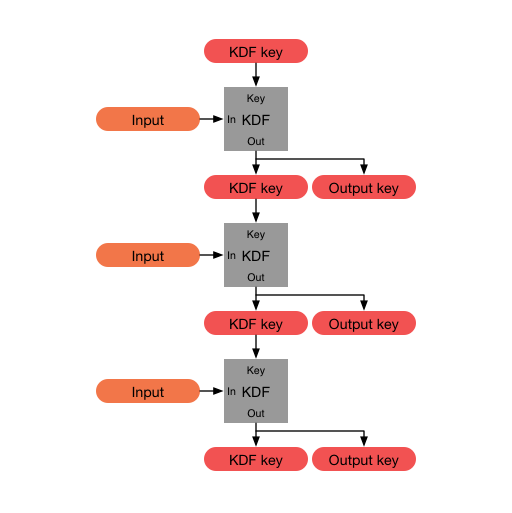
\includegraphics[width=0.8\textwidth]{ressources/kdf_chain.png}
  \caption{KDF Chain \parencite{perrin_double_2016}}
  \label{fig:KDF_Chain}
\end{figure}

\newpage
\subsubsection{Symmetric-key ratchet}

With the Symmetric-key ratchet, each message is encrypted with a unique message key. The message keys are generated with every ratchet step. In addition, a chain key is generated, which then can be used as a KDF key for the next ratchet step. The input, which can also be seen in figure \ref{fig:KDF_Chain}, is always a constant in the Symmetric-Key Ratchet, which means that if an attacker comes into possession of a chain key and the constant, he can decrypt subsequent messages. The message keys only ensure that each message is encrypted with a unique key and can theoretically be deleted after receiving the message. In addition, however, the respective keys contain a counter that allows the matching key to be found for the message, which could by chance not arrive in the order, in which they were sent. However, there is no security flaw in storing these message keys, because they are not used to generate other keys \parencite{perrin_double_2016}.


\subsubsection{Diffie-Hellman ratchet}
If an adversary could steal the transmitter and receiver chain keys, it would be possible for him to decrypt all messages in the future. To prevent this from happening, the Double Ratcheting Algorithm combines two different types of KDF chains. While the transmitter and receiver chains are based on symmetric Keychains, the root chain is a DH ratchet. The transmitter and receiver chains both use a DH-keypair from the root chain as starting point. With each message, the Symmetric-key ratchet is extended by one chain link. However, to ensure security for messages in the future, the symmetric Keychains' actual constant values are updated with the values from the DH ratchet, causing them to be reset. The root chain can always create new transmitter and receiver chains with new public keys. In the default implementation this happens with every message \parencite{perrin_double_2016}.

%\chapter{Problem definition}

\chapter{Analysis of the current situation}

When designing a new type of key management, it is important to look at the current solutions and their characteristics. This helps to have a better overview of the functions required in the concept. In addition, the concept should also provide a way to make it as easy as possible for the user to use his keys on several devices and thus have a simple administration of them. On the other hand, this step is also necessary to identify the problems of existing solutions so that they can be addressed.

\section{Use Cases for distributed Keys}

\subsection{Email}
One of the most used and oldest communication channels on the Internet is the e-mail. A great advantage, especially in the early days of the Internet, was that messages could be sent asynchronously. This means that the recipient could retrieve the message even if he or she was not online when it was sent, since the messages can be stored temporarily on a server \parencite{van_vleck_electronic_2012}. \newline
However, the e-mail as it was developed is more like a postcard than a letter. Anyone who receives it can also read it, since no form of encryption is provided. Most people, and therefore board members as well, do not use email encryption. Thus, important and confidential information is transmitted via this medium. Mostly people are not aware of the danger, how insecure the email is \parencite{managers_mail_2019}. \newline

In order to ensure the confidentiality and integrity of the messages, protocols such as SMIME or PGP were developed. These can ensure confidentiality by means of end-to-end encryption or integrity by means of a digital signature. Both solutions use the principle of public-key cryptography. However, even today most e-mails are neither signed nor encrypted, which is mainly due to the complicated setup. The creation of the key pairs is somewhat complicated for both standards. They are usually created offline on a local computer. The private keys must then be distributed to all computers that need access to them using one of the methods from \ref{sec:distribution}. The public keys must be distributed to all communication partners. Another possibility, as briefly mentioned in the basics, is to have the keys generated by a Certificate Authority, after which the keys must be distributed accordingly \parencite{kirsch_2001}.

In 2018 the so-called Efail vulnerability was revealed. The main cause were ActiveX elements that could be embedded in emails by an attacker during the mail transport. After the victim decrypted the email, the attacker was able to read the content using the ActiveX elements and send it where he wanted. In the meantime, most email clients have been updated and newer versions of the protocols have been adapted accordingly \parencite{bsi_bsi_nodate}.

\subsection{SSH}
SSH is a protocol that is mainly known through the remote administration of other computers and was also developed to replace other protocols like Telnet.  Beyond that, it is an independent, encrypted network protocol. It also allows other protocols like HTTP to be tunneled through SSH connections, which is practically equivalent to a VPN. Other protocols such as SCP for data transfer or Git as a distributed version management system are also based on it or use SSH for authentication. The authentication is usually done with passwords. Alternatively, authentication via public/private key is also possible, which makes it relevant for key distribution \parencite{luber_ssh_2020}.


\subsection{Password Manager}
Passwords are one of the most widely used types of authentication mechanisms on the Internet. Nearly every service uses them to verify that the user is the specified user by knowing that only the authorized user should have access to them. The problem that emerges is that there are many users who use weak passwords or who use the same password for several services. Both of these are security risks \parencite{verizon_2019}.

Therefore, there are password managers that are able to generate passwords securely and making them usable only with access to a master password and/or key file. The passwords of the services are stored in databases that are encrypted with the master password/keyfile. To be able to use all services on all devices, the password database must be distributed on several devices in the case of an offline password manager that does not store the data on the provider's servers. If a keyfile is used, it must also be securely distributed to multiple devices \parencite{reichl_composite_nodate}.

There are already other password managers that also use a smartphone as a kind of hardware security module. This requires a USB dongle that emulates a keyboard. If a service is accessed afterwards, only the required password has to be transferred to the computer and not the complete database of the password manager \parencite{noauthor_phraselock_nodate}.

\subsection{Multi-factor authentication}
The multi-factor authentication is an extension of the authentication as explained in the previous chapter by the password. In addition to the knowledge that a user must have in order to log in, the ownership of another device, for example, can be used as an additional authentication factor. 

\subsection{Crypto Currencies}
The principle of public-key cryptography is also used for cryptocurrencies like Bitcoin. This is used to generate signatures for transactions. 
The public key represents the receiving address, similar to the IBAN in bank communication. It can also be used to encrypt messages that only the recipient should be able to read. As a rule, however, there is not only one public-private key pair, but several, which are combined under a master key that encrypts all others as with the password manager. It is beyond the scope of this paper to look further into the background of the Master Key. However, if several devices should have access to the money, the master key must be distributed to several devices \parencite{btcecho_bitcoin_2018}.


\section{Distribution of private keys}
\label{sec:distribution}

\subsection{Local/Offline}
For example, to transfer a private key from one device to another, a USB cable can be used. For devices such as smartphones, a normal cable can be used for this purpose, which is also used to charge the smartphone. If one wishes to transfer a private key from a desktop computer to a laptop, for example, one must use a connection cable to enable the transfer \parencite{stiemer_linkkabel_2017}.

\subsubsection{USB stick}
Another way to exchange data securely could be the use of a USB stick, whereas this solution is more suitable for two different computers than the connection with smartphones. If the USB stick is trustworthy, there is no danger for the respective computers and the key can be transferred in this way. However, it should be noted that the data of the key is still stored on the USB stick, even if the key has been deleted on the computer. The memory cells are only marked for deletion and not directly overwritten. The data can be reconstructed with special software \parencite{bsi_bsi_loeschen}. \newline
As an additional security measure one could pack the key into an archive and protect it with a password. However, there is also the attack vector that attackers who come into possession of the USB stick can find out the password with a dictionary attack or brute force \parencite{rehim_effective_2016}.

\subsection{SCP}
As already mentioned, SCP is a protocol for exchanging data securely via SSH. It could also be used to transfer the private key. A positive aspect is that the connection is automatically encrypted and, compared to USB sticks, no data is left over that an attacker could use. The disadvantage is that an SSH connection must first be established, which is still easy on desktop operating systems. However, on iPhones it does not work without a jailbreak. The alternative for iPhones would be Airdrop, which is a proprietary service from Apple and not available on other operating systems which do not stem from Apple. How easy it is to use therefore depends on the devices that are supposed to participate in the communication \parencite{winscp_how_nodate}.

\subsection{Webservers/Downloads}
The possibility to create the private key at a CA also provides the potential to download it once on all devices via the web server of the CA. Since the connection is protected with HTTPS, this is also secure and user-friendly, since no separate servers have to be set up beforehand to start the file transfer. For this kind of transfer, only the known attacks for HTTPS would work. In addition, the server would have to carry out authentication, which again involves the risk of phising.

\subsection{External Providers}
Last but not least, there is the possibility to synchronize the private key with cloud providers like Google Drive or Dropbox on the different devices. However, this requires a great deal of trust in the cloud provider. In doing so, the legal regulations of the respective countries of origin must also be observed. Since the service may have to release the data at the request of the government \parencite{heise_us_nodate}. \newline
The user-friendliness is very high and the security is similar to that of web servers, as the transmissions are usually secured with HTTPS. In addition, there is also the risk that the login data can be tapped by means of phishing. Once the key has fallen into the hands of criminals, it is no longer usable. The biggest shortcoming, however, is the great trust that must be placed in the cloud provider. 


\section{Requirements for a Key-Service}
In order to create a new type of key distribution system, it is necessary to analyze what requirements are placed on such a system. For this purpose, the use cases are used to filter out an intersection of the requirements, which should then represent the cornerstones of the new application.

\subsection{Usability}
As the use cases have shown, a solution for the distribution of secrets must above all be user-friendly. If one takes a closer look at SCP, one will notice that it can only be used very differently on different operating systems and platforms or only with massive intervention in the system. The most convenient solution is therefore the cloud. Here, any device can access and use the secrets, with a minimal set-up effort for the user. Since most smartphone users have a Google or Apple account anyway, they also have a cloud service of the respective companies.

\newpage
\subsection{Security}
Considering the security, SCP is the best choice. The transmission is directly encrypted, there are no remnants of the secrets and no other parties are involved. The web server and cloud solutions are also technically secure. However, third parties must be trusted to treat user data confidentially.

\chapter{Concept}

\section{Architecture}
\label{sec:architecture}
\begin{figure}[ht]
	\centering
  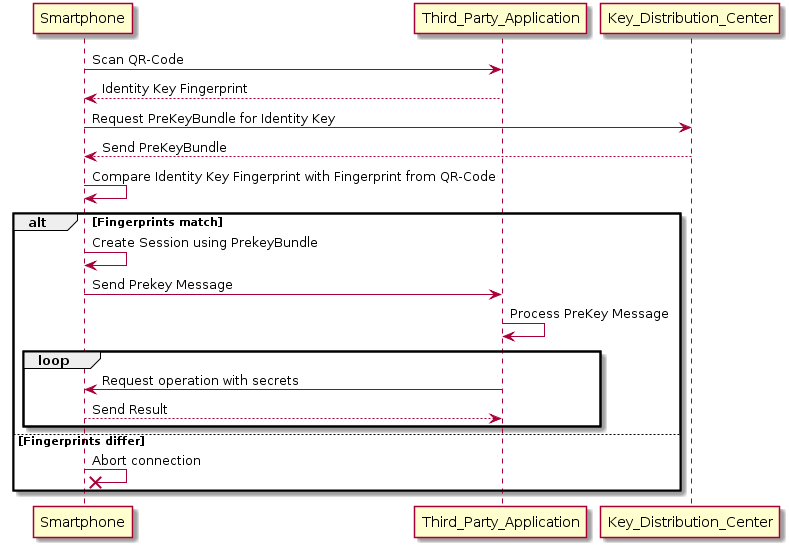
\includegraphics[width=0.8\textwidth]{ressources/process_flow.png}
  \caption{Application Flow (self-created representation)}
  \label{fig:app_flo}
\end{figure}
The figure shows the basic flow of the application. The Third-Party Application displays the fingerprint of it's own identity key in a QR-Code, which the smartphone can scan and thus receive the fingerprint of the third-party application. Using the fingerprint, the smartphone can then request a PreKeyBundle from the Key Distribution Center. Subsequently, the smartphone can check whether the fingerprint from the QR-Code matches that of the PreKeyBundle, since it is signed with the Identity Key. If this check fails, the smartphone terminates the communication. Otherwise, the smartphone can use the PreKeyBundle to create a PreKey Message which can be processed by the desktop application to establish a session. After these steps have been successfully completed, the application can make regular requests to the smartphone to perform cryptographic operations. 

The secrets that the third-party application wants to use are protected by the security mechanisms provided by the devices (Keychain or Keystore).
In case the secrets are private keys, all cryptographic functions that require the key must be executed on the mobile phone. Thus, the key does not have to be transferred and always remains on the smartphone. However, if a password manager is to be implemented, it cannot be avoided that the secret is transferred. 
At least the Third-Party Application should not save the secret, but this cannot be verified.

\section{Signal Protocol}
After an evaluation, as shown in \ref{tab:crypto_eval}, it has been found that the Signal Protocol is the best suited end-to-end encryption for such an application. A classical secure connection like in a client-server model, for example with HTTPS, would not be appropriate, because then more trust has to be put back into the server in the middle, which establishes the connections of the clients. Otherwise the server would be able to read all messages. Therefore, only protocols that offer end-to-end encryption can be considered.
\begin{table}[ht]
    \centering
    \setlength{\colw}{0.15\textwidth-2\tabcolsep}
    \begin{tabular}{L{0.39\textwidth-2\tabcolsep}||C{\colw}|C{\colw}|C{\colw}|C{\colw}}
        & \textbf{Weighting}& \textbf{Signal-Protocol} & \textbf{SMIME} & \textbf{OTR}  \\
        \hhline{=::====} Usability &
        3 & 2 & 1 & 2 \\
        \hline Platform independent & 2 & 3 & 3 & 2\\
        \hline Scalability & 1 & 3 & 3 & 3 \\
        \hline Verifiable security & 3 & 3 & 2 & 2 \\
    \end{tabular}
    \caption{Evaluation of the cryptography protocols}
    \label{tab:crypto_eval}
\end{table} \newpage
Usability is particularly important for the application. Both the actual user and other developers, who write plugins for other applications, should have it as easy as possible. With the Signal Protocol, there is a simple guide for the implementation, and once the classes for storing the secrets are written, a session can be established with a few lines of code.
With SMIME, the certificates would have to be signed by a CA first. Alternatively, they could be signed by everyone themselves, which would require separate keys for a CA. If neither of these is possible, independent authentication would have to be implemented, which is not practical.

Compared to Signal, OTR works without a Key Distribution Center, which is an advantage in this case, since no asynchronous communication is necessary anyway. However, there is no official implementation of the protocol, as there is no fixed institution behind the protocol. This can be good or bad depending on the point of view.

The signal library is available for Java, C and Javascript. SMIME is based on OpenSSL, which is also available on every system. OTR lacks an implementation for the Web, that is, Javascript.

Scalability plays a rather subordinate role in this application, as there are only 1:1 connections. However, intermediate stations, as required by the signal protocol, should not become a bottleneck. Considering how many millions of users Whatsapp serves, there will probably be no scalability complications with this type of application. SMIME only needs to rely on the normal mail servers, so it makes no difference whether encrypted or signed emails are sent or unencrypted or unsigned mails.

Since confidential information is to be transferred via the application, it is important that the protocol can be checked for security by independent researchers and that it passes this check.
With the signal protocol, there is a risk of a man-in-the-middle attack, if the fingerprint is not verified. In addition, an Unknown Key Share attack may occur. To exploit this, an attacker would have to be able to present his own QR code to the smartphone. This attack can only be minimized by adding unique information in the fingerprint, such as a clear name, telephone number or similar, but cannot be prevented \parencite{marlinspike_x3dh_2016}. \newline
SMIME had problems in the past with the E-Fail gap, which has been closed. However, the entire communication is readable for an attacker as soon as he knows the victim's private key since neither break-in nor future secrecy is possible with SMIME \parencite{bsi_bsi_nodate}. \newline
Also the OTR protocol had security flaws in previous versions like using a weak hash algorithm (SHA-1). Even if the security flaws of previous versions do not really affect the current version, they should still be noted. \parencite{bonneau_finite-state_nodate}.

\section{gRPC}
The way the architecture of the application is constructed suggests that the smartphone represents the server role, as it provides the cryptographic services. However, this would mean that the third-party application would make the request for decryption to the smartphone. But it cannot do this, because it does not know the address of the smartphone. While it would theoretically be possible, after scanning the QR-Code containing the address of the third-party application, to send a notification from the server to the third-party application, this increases the complexity and causes problems especially on Apple devices as servers on smartphones are normally not intended. Instead, it is easier for the third-party application to create a server which the smartphone can access. As shown in Figure \ref{fig:app_flo}. However, there must be a way for the server to send messages to the smartphone. This could be done through a Websocket connection or gRPC. While Websockets require additional manual identifiers to specify what the smartphone should do with the message, gRPC allows it to call another function directly.

Another possibility would be the use of WebRTC, which is mostly used for applications such as real-time video communication in the browser, since the protocol only needs both endpoints and no server for communication after the connection is established. This also makes the protocol very performant. Besides the video channels there is also the possibility to build a data channel that is interesting for this application.  Note, however, that a server is required for the initial connection setup to connect the respective end points. Although end-to-end encryption is also possible with WebRTC, since there are no intermediary entities, the signal protocol is not superfluous, as it offers authentication, forward and break-in secrecy. With gRPC offline communication in the same network is also possible.  Therefore, gRPC is very well suited for this application \parencite{badach_webrtc_2013}.

\section{Keychain/Keystore}
\subsection{Android}
For the application the version of Android 4.4 or higher is assumed, since the market share of lower versions together is less than 4\% \parencite{google_distribution_2019}. \newline
In addition, Android 4.0 introduced the Android Keystore Provider, which is required for the application and also introduced the facial recognition feature, which makes it likely that a TEE is present, but is not a guarantee. This can only be verified after a key has been generated. If no TEE is present, a software fallback of the Keystore is used \parencite{cooijmans_analysis_2014}.


There are different attack scenarios to get the keys in the Keystores as an attacker. For the different types of Keystores, it is therefore possible to examine which weak points arise for the respective attack scenario. 
\begin{itemize}
    \item Malicious app: Another app that has no exceptional rights is installed on the smartphone. However, it is assumed that the app has requested all rights it can get from the user like media access, camera or internet access.
    \item Root attack: The attacker controls an app on the smartphone that has gained root privileges. 
    \item Intercepting Root attack: In addition to the privileges of the root attack, the attacker can read the memory to retrieve user input. 
\end{itemize}

\textbf{Software Keystore:} \newline
Malicious App: Keys are protected by sandbox. \newline
Root Attack: Sandbox can be bypassed. Because the keys are stored with a password generated by the Keystore with read/write rights of the Keystore user, the password can also be read by a root user. So the keys can be used by another app as well as be viewed in plain text. This way the keys can also be transferred to another device. \newline If instead of the software fallback of the Android Keystore the Bouncycastle Keystore of Java is used together with a user password, the keys cannot be used without further ado. However, the use of this keystore must be explicitly specified in the source code.\newline
Intercepting Root Attack: In the case of the fallback solution, the result is the same as in the root attack. With Bouncycastle, the user's password input can be tapped and thus the keystore can be opened.\newline
\textbf{Hardware Backed Keystore:} \newline
Malicious App: Keys are protected by sandbox. \newline
Root Attack: Sandbox can be bypassed. The App identifier, which has access to the key material, can be adjusted so that another app can use the keys but cannot the keys in plaintext because they are bound to the hardware.\newline
Intercepting Root Attack: Same result as Root Attack \parencite{cooijmans_analysis_2014}.

Binding the keys to the hardware is especially important, because otherwise special hardware can be used that can guess the correct password faster than the smartphone.

In addition to the attack scenarios that are mainly based on the fact that an attacker has gained root privileges, there is also an attack that is based on security flaws in the frequently used Qualcomm processors. In this scenario, the full disk encryption of the device can be completely removed \parencite{laginimaineb_bits_2016}.

Since Android 7, however, it is no longer recommended and since Android 10 not possible anymore that the entire disk is encrypted with just one key. As another flaw was, that after the boot and decryption of the disk, all keys were remaining in the main memory. This is particularly critical because most users do not normally shut down their smartphones. Instead a file-based encryption is used, where individual files are encrypted. This also requires a built-in TrustZone \parencite{noauthor_filebased_nodate}.

In addition, the keys can be secured with a user authentication, such as a fingerprint or a password. It is not known to what extent securing the Keystores with user authentication will stop a root attacker.

The model of the StrongBox was primarily developed to better fend off so-called insider attacks. By this, Google means exploiting security holes that have already been installed by the hardware manufacturer or their suppliers \parencite{mayrhofer_insider_2019}.

There are no known vulnerabilities in the implementations of the StrongBox so far. However, it should be noted that only very few devices in the market have implemented the StrongBox and besides, except for the Google Pixel Smartphones, it is not really mentioned whether the device has a StrongBox or not.

Summarizing the results, it turns out that the solution should be preferred via the StrongBox if the device owns one. Depending on the application, it is probably also possible to work with the hardware-backed keys, since it is at least only possible to export the keys with a very high effort. However, if only the software keystore is available as fallback, an attacker with root privileges is able to export the keys directly to another device.
What is an advantage on the one hand, is a disadvantage on the other hand. If the keys are created hardware-bound, no backups of the keys can be created with normal means, because the developer never has the private key available. This means that if the device is exchanged, a new key must also be generated. Additionally, the keys are also deleted when the app is uninstalled.

To avoid the problem with root privileges, banks in particular rely on algorithms that detect whether the device has been rooted. In practice, however, there are also mechanisms to bypass exactly this detection to be able to use the app anyway. So it resembles an arms race who can trick whom. \parencite{mulliner_safetynet_2017}
% Der Key wird verschlüsselt in der unsicheren Welt abgespeichert, wird also nicht direkt im TEE abgespeichert
% Device Bound besonders wichtig wegen FPGA
% Seit ANdroid 10 keine Full Disk Encryption mehr sondern File Based
% Strongbox nur bei 

% ios Forensic
%https://www.elcomsoft.de/news/730.html 
\subsection{iOS}
In iOS, it is possible to generate keys either in memory or via the Secure Enclave. Again, there is a risk that if the key is loaded into the unsecured memory, it could be compromised. On the other hand, the Secure Enclave has the disadvantage that only 256-bit elliptic curve key pairs can be generated. It is also not possible to import RSA keys that were created in memory. So if other keys are used, the path must be taken via the RAM and thus the Keychain. Since iOS version 4 Apple also uses a kind of File Based Encryption to encrypt all data on a device. A separate key is created for each file. These keys are then stored on the disk in an insecure way, but are encrypted with a separate class key consisting of the user password and a unique hardware ID that is built into the processor. If additionally, the high security protection class is used, the class key is only available when the device is unlocked. If the lock screen is activated, the class key is deleted from the main memory. So it should be specified that the key should only be created or saved using the high security protection class.
While the KDF function actually offers good protection and Apple apparently cannot break the full encryption of the memory, an exploit was released at the end of 2019 that works for many iPhones and cannot be fixed with software updates.  To utilize the exploit, however, the attacker needs physical access to the system and after a reboot it would have to be performed again. However, the exploit does not affect the Secure Enclave where the TouchId is stored. So if the keys are encrypted using the TouchId, the attacker cannot access the keys even then \parencite{reed_new_2019}. \newline
Forensic software, which may only be used by authorities, advertises the possibility of using jailbreaks to make passwords, keys and decrypting the file system possible \parencite{coltd_elcomsoft_nodate}.

So theoretically it would be possible to synchronize the generated keys with the iCloud. However, this would again involve the security risks already explained, such as the trust in Apple, a cloud solution. In addition, Apple's Keychain application only works with other Apple devices. So the recommended storage is to use the Keychain for non-elliptic keys. Thereby, the synchronization by the iCloud should not be used. If the keys are elliptic curve keys, the secure enclave can be used and thus be bound to the hardware.

\section{Usability}
As already mentioned in \ref{sec:architecture}, the connection from the smartphone to the third-party application is established using a QR-Code. As soon as the smartphone has registered with the application as an HSM device, communication can immediately begin. In addition, a dialog should appear on the smartphone which key or secret the third-party application should have access to. If the session has ended, the connection is terminated. If a new connection is desired, a QR-Code must be scanned again.

\chapter{Implementation}

\section{Kotlin}
Kotlin is a programming language that is usually converted into bytecode for the Java Virtual Machine. The language is mainly developed by the IDE specialists Jetbrains. A main feature of the language is the ability to be compiled for different applications. For example, there is the possibility to compile from code written in Kotlin to Javascript code. It is also possible to compile libraries for iOS and Android with the same code base. The language first appeared on the market in 2016, although it has only been available in a stable version since 2016. In 2017 Kotlin was officially supported for Android applications by Google and since 2019 it is Google's preferred programming language for Android apps. 
The language is therefore well suited for the prototype, as it can be used both on the smartphone and on the desktop \parencite{lovis_ist_nodate}.

\section{gRPC}
As the concept pointed out, the architecture of the application can be well mapped with gRPC. However, the prototype should be limited to the most necessary. Therefore, in this case the Key Distribution Center can be omitted. Instead, the smartphone and the desktop application can exchange the key packages directly with each other. It should be noted that this must allow both devices to have a direct connection with each other. They must therefore be in the same network or be routed to each other. 

\section{Prototype}
With the help of the developed concept, a prototype can be developed which also serves as a proof of concept. Since the analysis of the current situation has shown that especially the key management in the field of email signing or encryption is difficult, this use case shall serve as a prototype. 

\subsection{App}
The prototype should show that a key can be generated on the smartphone that is suitable for SMIME. With this key it should then be possible to either sign or decrypt messages that a third-party application sends to the smartphone. Since encrypting or verifying messages does not require the own private key, these functions can be disregarded, since they can also be performed by a SMIME-enabled email client. 

\begin{lstlisting}[label=lst:keyparams,
				   language=java,
				   firstnumber=1,
				   caption=Creating an RSA key pair]

fun generateKeyPair() {
    val start = Calendar.getInstance()
    val end = Calendar.getInstance()
    end.add(Calendar.YEAR, 5)
    
    KeyPairGenerator.getInstance(
        KeyProperties.KEY_ALGORITHM_RSA,
        keyStoreProvider
    ).apply {
        val certBuilder = KeyGenParameterSpec.Builder(
            keyAlias,
            KeyProperties.PURPOSE_ENCRYPT or
                    KeyProperties.PURPOSE_DECRYPT or
                    KeyProperties.PURPOSE_VERIFY or
                    KeyProperties.PURPOSE_SIGN
        )
            .setUserAuthenticationRequired(true)
            .setKeySize(4096)
            .setKeyValidityEnd(end.time)
            .setKeyValidityStart(start.time)
            .setDigests(KeyProperties.DIGEST_SHA512)
            .setCertificateSerialNumber(BigInteger.ONE)
            .setCertificateSubject(X500Principal(principalName))
            .setSignaturePaddings(KeyProperties.SIGNATURE_PADDING_RSA_PKCS1)
            .setEncryptionPaddings(KeyProperties.ENCRYPTION_PADDING_RSA_PKCS1)

        if (Build.VERSION.SDK_INT >= Build.VERSION_CODES.P) {
            initialize(
                certBuilder
                    .setIsStrongBoxBacked(true)
                    .build()
            )
        } else {
            initialize(certBuilder.build())
        }
    }
}

\end{lstlisting}

Listing \ref{lst:keyparams} shows how an RSA key is created via the AndroidKeystoreProvider. Parameters such as the period of validity or the key length can also be specified here. A special security feature can be set with the option "setUserAuthenticationRequired(true)". This means that when the app accesses the key, the user must authenticate himself separately with stored features such as a pin or his fingerprint. Additionally, the Android version can be read out to check if there is a possibility that the device has a StrongBox.

\begin{lstlisting}[label=lst:session,
				   language=java,
				   firstnumber=1,
				   caption=Creating a Session]
fun startCommunication(qrCode: String) {
    serverAddress = qrCode.split("|")[0]
    val scannedFingerprint = qrCode.split("|")[1]

    val ownPreKeyPair = Curve.generateKeyPair()
    val ownSignedPreKeyPair = Curve.generateKeyPair()
    val ownSignedPreKeySignature = Curve.calculateSignature(
        signalProtocolStore.identityKeyPair.privateKey,
        ownSignedPreKeyPair.publicKey.serialize()
    )

    val ownPreKeyBundle = PreKeyBundle(
        signalProtocolStore.localRegistrationId, 1,
        SecureRandom().nextInt(),
        ownPreKeyPair.publicKey,
        SecureRandom().nextInt(),
        ownSignedPreKeyPair.publicKey,
        ownSignedPreKeySignature,
        signalProtocolStore.identityKeyPair.publicKey
    )

    val desktopKeyBundle = GrpcClient.instance.exchangeKeybundles(ownPreKeyBundle)
    if (desktopKeyBundle.identityKey.fingerprint != scannedFingerprint) {
        return
    }

    sessionBuilder.process(desktopKeyBundle)

    KeyTool().generateKeyPair()

    GrpcClient.instance.startCommunication()
}
\end{lstlisting}

The function shown in listing \ref{lst:session} shows the creation of the connection between smartphone and desktop client. The method is called by an Android Activity that scans a QR-Code which, in the case of the prototype, consists of the network address of the third-party device and its Prekey Bundle fingerprint. In order to establish the encryption, a Prekey Bundle is generated each time, which is exchanged. Then the app checks if a key pair already exists for the requested application. If it does not, it is generated as shown in listing \ref{lst:keyparams}. If needed, the App can create a \nameref{sec:CSR} to let a \nameref{sec:CA} sign the public key.

Depending on which functions are requested, functions such as signing or decrypting messages can then be called. 

To enable the cryptographic functions such as the generation of a signature in Android it needs a cryptography library. Android itself uses Bouncycastle in the background. This is only available in a slimmed down version in which functions like SMIME are not available. To be able to use these functions, there are providers like Spongycastle, which were adapted for Android. Unfortunately, this library could not be used without further ado, because it was still referenced to packages that exist in a normal Java installation, but not in Android. To use the functions anyway, the library has to be adapted regarding the mail functionality and added to the application \parencite{noauthor_bouncycastle_nodate}.

\subsection{Desktop Client}
The prototype for the third-party application has several functions to fulfill. The most important one is to create the server and generate the QR-Code. In addition, as mentioned, being a Certificate Authority. To simulate a user who wants to view different mails, every 20 seconds a file is read from the file system, which was previously encrypted using the public key generated on the smartphone. This file is then sent to the smartphone, decrypted and then displayed in plain text in the server console. 

\begin{lstlisting}
override fun subscribeMails(responseObserver: StreamObserver<MailRequest>?): StreamObserver<MailResponse?> {
    observer = responseObserver
    
    return object : StreamObserver<MailResponse?> {
        override fun onNext(value: MailResponse?) {
            if (!value?.mail?.isEmpty!!) {
                if (SessionGenerator
                .instance
                .signalProtocolStore
                .containsSession(SessionGenerator.instance.MOBILE_ADDRESS)) {
                    val message = SignalMessage(value.mail?.toByteArray())
                    val plaintext = SessionGenerator.instance.sessionCipher.decrypt(message)
                    if (String(plaintext) != "Das ist eine Testmail") {
                        println("Signatur ist korrekt?: ${verifySignature(plaintext)}")
                    } else
                        println(String(plaintext))
                } else {
                    val message = PreKeySignalMessage(value.mail?.toByteArray())
                    println(String(SessionGenerator.instance.decryptMessage(message)))
                }
            }
    
            val message = messages.firstOrNull()
            if (message != null) {
                val encryptedMessage = SessionGenerator.instance.sessionCipher.encrypt(message.mail.toByteArray())
    
                val mailRequest = MailRequest.newBuilder()
                        .setMail(ByteString.copyFrom(encryptedMessage.serialize()))
                        .setMethod(message.method)
                        .build()
                messages.remove(message)
                observer?.onNext(mailRequest)
            }
        }
    
        override fun onError(t: Throwable?) {
            println("error on server")
            t?.printStackTrace()
        }
    
        override fun onCompleted() {
            println("Completed on Server")
        }
    }
}
\end{lstlisting}

In addition, the prototype has functions such as requesting the decryption or signing of a mail and the sending of a mail.
% Nach dem verbinden mit QR Code könnte in der App eine Pin angezeigt werden die dann am PC eingegeben werden muss.


%\chapter{Evaluation}

%\section{Usability}

%\section{Security}

%\section{Existing Solutions}

%\section{QR-Based Solution}

\chapter{Review}
\section{Conclusion}
The thesis should deal with how the security mechanisms of iOS and Android can be used to use the smartphone as a hardware security module. In addition, a way to transport the application data as secure as possible from possible third-party applications to the smartphone had to be found. Especially the complicated key management of SMIME on different devices has shown that current methods are too complicated to be used. Therefore, the usability of the service was a very important feature that had to be fulfilled.

Since the data processed by a hardware security module is particularly worth protecting, as little trust as possible in third parties should be necessary to use the service. The result was that there is a server that establishes the connections and exchanges messages from the third-party application and smartphone. However, it is important to note that a malicious server could exchange a maximum of wrong messages or key bundles. Most importantly, the server is not able to read the actual messages, so end-to-end encryption was required. 

Furthermore, it was analyzed how the encrypted messages can be transmitted best. It turned out that both gRPC and WebRTC are suitable as possible protocols. gRPC was chosen for the solution because it does not necessarily require a server to establish the connection, but can also function in an encapsulated form from the Internet. If the Internet connection is taken for granted, WebRTC would be the better choice, as it is more performant and does not require a server once the connection is established. 

Afterwards it turned out that in the past, especially with Android, there were problems with the storage of the keys. Most of the problems were due to the fact that a user can gain root privileges, which is not provided for in the Android rights system. At Apple there are significantly fewer known security problems. However, this is certainly also due to the fact that it is more attractive for security researchers to investigate a system which is open source and does not have to be reverse-engineered first as is the case with Apple.

The prototypical implementation has shown that such an application is definitely possible. However, it has also been shown that support for SMIME from libraries within Android is certainly expandable, probably due to the low adoption of SMIME. 
\section{Outlook}
Since in the work mainly the email encryption with SMIME was considered as an example of use, other use cases should also be examined. First, it can be considered if it really makes sense to create the keys hardware-bound for each use case, because a backup of the keys is impossible. It is also very important that at least the communication specifications between app and third party application are clearly defined and publicly available, otherwise further development with other applications and protocols is not possible.

\backmatter
%%%%%%%%%%%%%%%%%%%
%% create figure list
%%%%%%%%%%%%%%%%%%%

\listoffigures
\addcontentsline{toc}{chapter}{Directories}

%%%%%%%%%%%%%%%%%%%
%% create tables list
%%%%%%%%%%%%%%%%%%%
% \listoftables

%%%%%%%%%%%%%%%%%%%
%% create listings list
%%%%%%%%%%%%%%%%%%%
%\lstlistoflistings
%\addcontentsline{toc}{chapter}{Listings}

\cleardoublepage
\phantomsection
\addcontentsline{toc}{chapter}{Bibliography}
\printbibliography

%%%%%%%%%%%%%%%%%%%
%% declaration on oath
%%%%%%%%%%%%%%%%%%%

\addchap{Affidavit}

I hereby certify that I have written my bachelor thesis independently and have not yet submitted it for examination purposes elsewhere. All sources and aids used are listed, literal and meaningful quotations have been marked as such.

\vspace{20pt}
\begin{flushright}
$\overline{~~~~~~~~~~~~~~~~~\mbox{\ShowBaAuthor, am \today}~~~~~~~~~~~~~~~~~}$
\end{flushright}

\addchap{Consent to plagiarism check}

I hereby agree that my submitted work may be sent to PlagScan (www.plagscan.com) in digital form for the purpose of checking for plagiarism and that it may be temporarily (max. 5~years) stored in the database maintained by PlagScan as well as personal data which are part of this work may be stored there.

\begin{small}
This Consent is voluntary. Without this consent, the plagiarism check can still take place, when all personal data is removed from the document. Consent to the storage and use of personal data may be revoked at any time by notifying the faculty.
\end{small}

\vspace{20pt}
\begin{flushright}
$\overline{~~~~~~~~~~~~~~~~~\mbox{\ShowBaAuthor, am \today}~~~~~~~~~~~~~~~~~}$
\end{flushright}

\end{document}
